\documentclass[11pt,a4paper]{article}

\usepackage[T1]{fontenc}
\usepackage[utf8]{inputenc}
\usepackage[english]{babel}
\usepackage[a4paper,margin=2.4cm]{geometry}
\usepackage{xcolor}
\usepackage{booktabs}
\usepackage{enumitem}
\usepackage{parskip}
\usepackage{fancyhdr}
\usepackage{csquotes}
\usepackage{tikz}
\usetikzlibrary{positioning, arrows.meta}
\usepackage[hidelinks]{hyperref}

% ---- colors --------------------------------------------------------------
\definecolor{ink}{HTML}{1B2733}
\definecolor{accent}{HTML}{2F6FB0}
\definecolor{keybg}{HTML}{E9F2FB}
\definecolor{warnbg}{HTML}{FBEEE0}
\definecolor{tipbg}{HTML}{E9F6EE}
\definecolor{up}{HTML}{DCE9F7}
\definecolor{scen}{HTML}{DDF0E3}
\definecolor{ana}{HTML}{EADCF3}
\definecolor{eval}{HTML}{F7E7D6}

\hypersetup{colorlinks=false, pdftitle={DiLab Foresight Pipeline — Required Reading},
  pdfauthor={DiLab Foresight Team}}

% ---- callouts (robust: colorbox + parbox, no extra packages) -------------
\newcommand{\callout}[3]{\par\smallskip\noindent
  \colorbox{#1}{\parbox{\dimexpr\linewidth-2\fboxsep\relax}{%
  \textbf{#2}\\[2pt]#3}}\par\smallskip}
\newcommand{\key}[2]{\callout{keybg}{#1}{#2}}
\newcommand{\warnb}[2]{\callout{warnbg}{#1}{#2}}
\newcommand{\tipb}[2]{\callout{tipbg}{#1}{#2}}
\newcommand{\code}[1]{\texttt{\small #1}}

\pagestyle{fancy}
\fancyhf{}
\lhead{\small\textcolor{accent}{DiLab Foresight}}
\rhead{\small Required Reading}
\cfoot{\small\thepage}
\renewcommand{\headrulewidth}{0.4pt}

\setlist[itemize]{leftmargin=1.4em, itemsep=2pt, topsep=3pt}
\setlist[enumerate]{leftmargin=1.6em, itemsep=2pt, topsep=3pt}

\title{\vspace{-1.2cm}\textbf{How Our Foresight Pipeline Works}\\[4pt]
  \large Required reading \textit{before} you build slides}
\author{DiLab Foresight Team}
\date{As of 8 July 2026}

\begin{document}
\maketitle
\thispagestyle{fancy}

\begin{abstract}
\noindent This document explains, \textbf{from scratch and assuming no prior knowledge}, what our
pipeline does, why it is built this way, and -- most importantly -- \textbf{what our actual result is}.
Read it fully before making slides. At the end you will find a glossary and a list of
\enquote{sentences you must never say}. If you only have five minutes, read Section~1 (the big picture)
and Section~7 (the central finding).
\end{abstract}

\tableofcontents
\vspace{4mm}

% =========================================================================
\section{What is this even about?}

We are \textbf{not} building a tool that \enquote{predicts the future}. We are building a
\textbf{foresight pipeline}: an automated machine that turns a collection of documents
(\enquote{what do we know about this field?}) into a \textbf{map of plausible futures} --
structured, traceable, and without a human having to invent the scenarios by hand.

Two things are central and should appear in every presentation:

\begin{itemize}
  \item \textbf{Domain-agnostic.} The actual product is a \emph{generic} framework. You dock any
  knowledge base onto it (spectrum monitoring, agriculture, whatever) and the pipeline derives the rest
  by itself. \emph{Spectrum monitoring is only our test case} (the sponsor, Rohde \& Schwarz), not the
  purpose.
  \item \textbf{Traceability.} Every statement, every driver, every scenario carries references
  (\code{source\_chunk\_ids}) back to the concrete passages in the knowledge base. Nothing is
  \enquote{hallucinated} without a source you can look up.
\end{itemize}

\key{The one-sentence explanation}{The pipeline reads a knowledge base, distills the \emph{driving
uncertainties} of a field, spans a space of plausible scenarios from them, and evaluates that space
honestly -- including the question of whether clear \enquote{archetypes} exist at all, or only a
continuum.}

% =========================================================================
\section{The mental model (big picture)}

Before the individual steps, the picture to hold in your head. Everything splits into four phases:

\begin{enumerate}
  \item \textbf{Upstream (what is the world made of?)} -- \emph{drivers} are extracted from documents and
  their possible states are defined.
  \item \textbf{Scenario generation (which combinations are coherent?)} -- the drivers are coupled
  (which one promotes/inhibits which?) and coherent combinations = scenarios are produced. We do this
  with \emph{two} methods in parallel.
  \item \textbf{Analysis (what structure does the scenario space have?)} -- are there clearly separable
  groups (\emph{archetypes}) or is everything a gradual transition (\emph{continuum})? This is where our
  main finding lives.
  \item \textbf{Evaluation \& synthesis (what does it mean strategically?)} -- scenarios are scored
  (multi-criteria), placed in time, and summarized strategically.
\end{enumerate}

\begin{figure}[h]
\centering
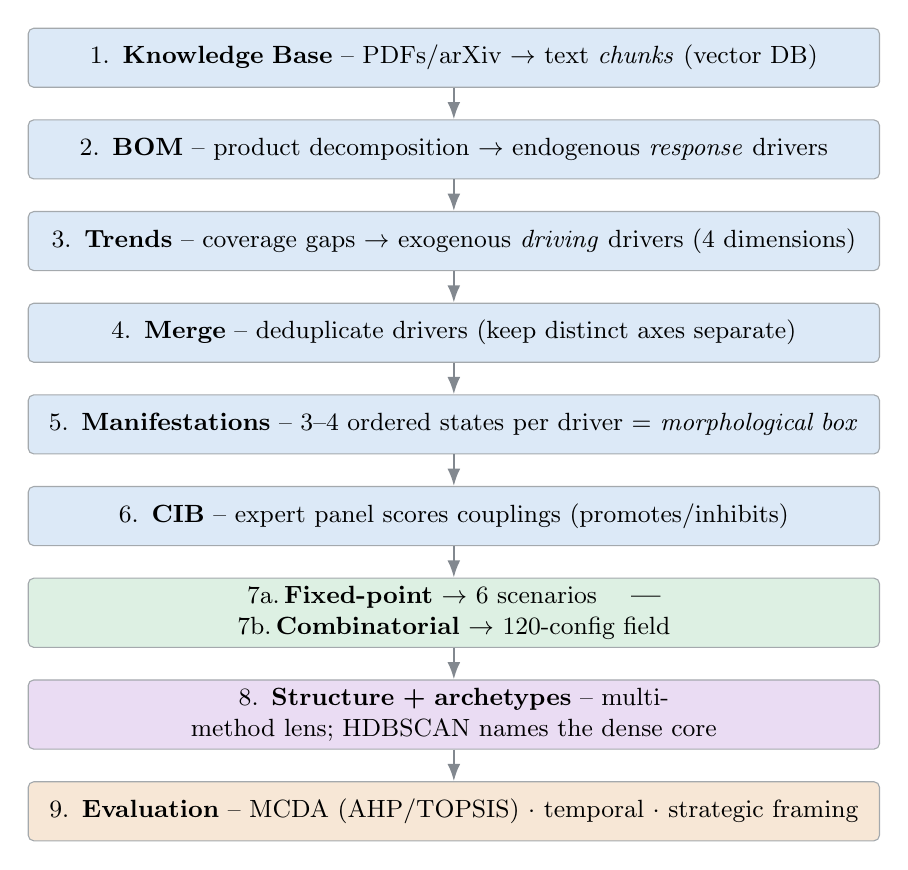
\begin{tikzpicture}[
  font=\small,
  box/.style={draw=ink!40, rounded corners=2pt, text width=10.6cm, align=center,
              minimum height=7.5mm, inner sep=3pt},
  arr/.style={-{Latex[length=2.2mm]}, thick, ink!55}]
  \node[box, fill=up]   (kb)   {1. \textbf{Knowledge Base} -- PDFs/arXiv $\to$ text \emph{chunks} (vector DB)};
  \node[box, fill=up, below=4mm of kb] (bom) {2. \textbf{BOM} -- product decomposition $\to$ endogenous \emph{response} drivers};
  \node[box, fill=up, below=4mm of bom] (tr) {3. \textbf{Trends} -- coverage gaps $\to$ exogenous \emph{driving} drivers (4 dimensions)};
  \node[box, fill=up, below=4mm of tr] (mg) {4. \textbf{Merge} -- deduplicate drivers (keep distinct axes separate)};
  \node[box, fill=up, below=4mm of mg] (mf) {5. \textbf{Manifestations} -- 3--4 ordered states per driver = \emph{morphological box}};
  \node[box, fill=up, below=4mm of mf] (cib) {6. \textbf{CIB} -- expert panel scores couplings (promotes/inhibits)};
  \node[box, fill=scen, below=4mm of cib] (sc) {7a.\,\textbf{Fixed-point} $\to$ 6 scenarios \quad\textbf{|}\quad 7b.\,\textbf{Combinatorial} $\to$ 120-config field};
  \node[box, fill=ana, below=4mm of sc] (an) {8. \textbf{Structure + archetypes} -- multi-method lens; HDBSCAN names the dense core};
  \node[box, fill=eval, below=4mm of an] (ev) {9. \textbf{Evaluation} -- MCDA (AHP/TOPSIS) $\cdot$ temporal $\cdot$ strategic framing};
  \draw[arr] (kb)--(bom); \draw[arr] (bom)--(tr); \draw[arr] (tr)--(mg);
  \draw[arr] (mg)--(mf); \draw[arr] (mf)--(cib); \draw[arr] (cib)--(sc);
  \draw[arr] (sc)--(an); \draw[arr] (an)--(ev);
\end{tikzpicture}
\caption{The data flow. Blue = upstream, green = scenario methods, purple = analysis, orange = evaluation.}
\end{figure}

\key{The single most important concept: driving vs.\ response}{We separate \textbf{driving axes}
(exogenous uncertainties of the \emph{environment} -- regulation, market, geopolitics, technology push)
from \textbf{response axes} (the actor's own product/technology, e.g.\ hardware/software).
\textbf{Scenarios are spanned by the driving axes}; the technology is what \emph{responds} and gets
evaluated per scenario. Whoever mixes these two up explains the whole method wrong.}

% =========================================================================
\section{The pipeline step by step}

\subsection{Knowledge Base (KB)}
All source PDFs and arXiv papers are split into small text \emph{chunks}, turned into vectors
(\emph{embeddings}) and stored in a vector database (Chroma). Currently $\approx$3{,}900 chunks for the
spectrum test case. Each chunk has a \code{pool}: \code{product} (describes our product) or \code{trend}
(describes the environment). This is the only docking point -- everything else is derived.

\subsection{BOM -- the product decomposition}
BOM = \emph{Bill of Materials}. The R\&S product is decomposed into its building blocks (ADC, digital
downconverter, direction-finding modules, \dots). These become \textbf{response drivers} -- they are the
\emph{system} under study, not the driving uncertainty.

\subsection{Trends -- driving uncertainties from the coverage gaps}
Here is an elegant idea: a trend chunk is interesting exactly when \emph{none} of the BOM building blocks
already covers it (similarity below a threshold). Such chunks are called \textbf{orphans} -- they describe
environment the product does not yet capture, i.e.\ potential \emph{driving} uncertainties. Flow:
\begin{enumerate}
  \item Each orphan is assigned to its nearest \textbf{driving dimension}: \emph{regulatory, market,
  geopolitical, technological} (generic, domain-neutral anchors).
  \item Within each dimension we cluster; granularity scales with how much content that dimension has
  (a rich dimension $\to$ more, more distinct drivers).
  \item An LLM formulates one driver per cluster and \textbf{stamps} its dimension onto it.
\end{enumerate}
\textbf{Source cap:} no single document may contribute more than $N$ chunks (currently 150) to the orphan
pool. Without it, two huge regulatory documents (WRC-23, ITU Handbook) would drown everything else.

\subsection{Merge -- consolidate, but keep the axes apart}
BOM and trend drivers are deduplicated (same names, similar embeddings, LLM grouping). New and important:
a \textbf{cross-dimension guard} prevents drivers of \emph{different} dimensions from being merged
together. Afterwards each driver has an \code{axis\_role} (driving/response). For the expensive CIB step
the \textbf{top 14} drivers are selected (weighted by origin + amount of evidence).

\subsection{Manifestations -- the morphological box}
For each driver an LLM generates 3--4 \textbf{states} (manifestations), \emph{ordered} from optimistic to
pessimistic. Drivers $\times$ states = the \textbf{morphological box} (\emph{Zwicky box}). A \emph{scenario}
is simply: pick exactly one state from each driver.

\subsection{CIB -- Cross-Impact Balance (the heart)}
CIB (after Weimer-Jehle) asks, for \emph{every pair of drivers}: \enquote{If driver A takes this state --
does that promote (+) or inhibit (-) a particular state of driver B?} Instead of a single opinion we use
a \textbf{panel of several AI personas} + two \emph{Delphi} rounds (the personas see the outliers and may
revise). Two specifics:
\begin{itemize}
  \item \textbf{Dissent-preserving:} if a minority sees a strong trade-off (score $\le -2$), it is
  \emph{not} averaged away by the median. Reason: LLMs are too positive; without this we would get almost
  only \enquote{everything promotes everything} and the scenario space collapses.
  \item \textbf{Calibration:} we measure the share of negative entries in the matrix. $\approx$24\,\%
  negative sits in the literature-normal range (20--30\,\%). Before, it was near 0\,\% -- a known LLM
  positivity bias.
\end{itemize}

\subsection{Two routes to scenarios (deliberately parallel)}
From the box + CIB matrix, scenarios are produced in \textbf{two} ways -- both kept as equal-standing
views:
\begin{itemize}
  \item \textbf{7a. Fixed-point method (classic Weimer-Jehle).} Find \emph{self-consistent equilibria}:
  configurations where no single driver \enquote{wants to flip}. These are the \textbf{fixed points}
  (attractors). From them, 6 maximally different, typed scenarios are chosen.
  \item \textbf{7b. Combinatorial method.} Instead of the hard fixed-point gate, a \emph{soft} filter (a
  \enquote{contradiction ratio}): sample $\approx$120 plausible configurations. This yields a \emph{whole
  field} instead of a few points -- the basis for the archetype analysis.
\end{itemize}
For each configuration an LLM writes a \textbf{grounded narrative} (with RAG evidence from the KB).

\subsection{Landscape -- the map}
The scenario space is visualized (UMAP for looks, PCA for \emph{interpretable} axes) and annotated with an
honest structure verdict (see Section~\ref{sec:structure}).

\subsection{Evaluation, time, strategy}
\begin{itemize}
  \item \textbf{Grounded evaluation / MCDA:} an evidence-based auditor scores each scenario along several
  criteria (impact, probability, actionability, time horizon, risk), \emph{with evidence} per score. MCDA
  (AHP weights + TOPSIS ranking) turns this into a ranked list.
  \item \textbf{Temporal / DVI:} places drivers by signal maturity (emerging vs.\ established).
  \item \textbf{Strategic framing:} an LLM synthesizes the whole analysis into strategic statements.
\end{itemize}

% =========================================================================
\section{Why TWO scenario methods?}

They answer different questions and share the same upstream (KB $\to$ drivers $\to$ CIB) and the same
downstream (narratives $\to$ landscape $\to$ evaluation). Only the selection step differs.

\begin{center}\small
\begin{tabular}{@{}p{3.1cm}p{5.3cm}p{5.3cm}@{}}
\toprule
 & \textbf{Fixed-point (7a)} & \textbf{Combinatorial (7b)} \\
\midrule
Question & Where does the system \emph{rest}? (equilibria) & What is plausible at all? (whole field) \\
Filter & hard (true fixed points) & soft (contradiction ratio) \\
Output & few (6) typed scenarios & large field ($\approx$120) \\
Strength & classic, established, comparable & basis for clusters/archetypes \\
\bottomrule
\end{tabular}
\end{center}

\tipb{Framing for the slides}{\enquote{We offer the classic Weimer-Jehle fixed-point analysis \emph{and} a
field-based combinatorial analysis -- both from the same, computed-once upstream.} That is credible and
honest.}

% =========================================================================
\section{Structure: are there archetypes or a continuum?}\label{sec:structure}

The dream of every scenario study: \enquote{here are the 3--4 archetype scenarios.} But you may only claim
that if the space \emph{actually} splits into separable groups. So we measure it instead of asserting it.

\textbf{Silhouette \& null model.} The \emph{silhouette} measures (0--1) how cleanly separated clusters
are. Rule of thumb: below \textbf{0.25} = no usable clusters. We additionally compare against a
\textbf{uniform-random null model} (same field, but randomly filled): is our structure significantly
larger than pure chance?

\textbf{Multi-method lens.} The crux: the standard method (KMeans) \emph{forces every point into a cluster}
and thereby misses structure. So we look through several \enquote{lenses}:
\begin{itemize}
  \item Encoding: \emph{one-hot} vs.\ \emph{ordinal} (ordinal keeps the optimistic$\to$pessimistic order).
  \item Method: \emph{KMeans} (all points) vs.\ \emph{HDBSCAN} (density-based, allowed to leave points as
  \enquote{noise}, unclustered).
\end{itemize}

\warnb{Do not compare apples with oranges}{The HDBSCAN silhouette applies only to the \emph{dense part}
(noise excluded) and is \textbf{not} directly comparable to the KMeans silhouette (all points). On slides,
always put them side by side -- do not sell it as \enquote{we improved the silhouette from 0.07 to 0.4}.}

% =========================================================================
\section{The central finding (this must stick)}

After all improvements (more \& more independent drivers, a de-skewed corpus, a de-biased CIB), the honest,
measured result is:

\key{The field is a HYBRID}{It is \textbf{neither} a cleanly clustered space \textbf{nor} pure chaos, but a
\textbf{dense archetypal core} (a minority of scenarios form real, well-separated groups) \textbf{embedded
in a continuum} (the majority blend gradually into one another). Standard KMeans hid the core;
\textbf{HDBSCAN + ordinal encoding} reveal it.}

Concretely (spectrum test case, combinatorial field, 120 configurations):
\begin{itemize}
  \item KMeans over all points: silhouette $\approx$0.07 (looks like \enquote{no structure}).
  \item HDBSCAN + ordinal: finds \textbf{7 dense clusters} (silhouette $\approx$0.39); $\approx$37\,\% of
  points remain as a \emph{continuum halo}, unclustered.
  \item These 7 clusters are \textbf{named} by an LLM (e.g.\ \enquote{Assured Spectrum Commons},
  \enquote{Contested Sharing Governance}, \enquote{Algorithmic Spectrum Stewardship}, \dots), each with the
  driver states that distinguish it from the others.
\end{itemize}

\textbf{Why is the engine nonetheless correct (and why that is our selling point)?} We have a
\emph{positive control}: an artificial field with \emph{genuine} block structure yields silhouette
$\approx$0.72 -- the machine \emph{does} find clear clusters when they exist. Our real field looks
different because the domain is that way, not because the tool fails. \textbf{The engine measures the input
property honestly and does not hallucinate clusters.} That integrity is exactly the point.

% =========================================================================
\section{Honest limitations (state them proactively)}
\begin{itemize}
  \item \textbf{Continuum halo:} the archetypes describe the \emph{core}, not the whole space. Always quote
  the halo's percentage.
  \item \textbf{Corpus skew:} the geopolitical dimension is still thin (1--2 drivers). Enriching it with
  more / opposing sources is on the roadmap.
  \item \textbf{MCDA compression:} the evaluation LLM often gives very similar scores (impact/probability
  barely spread). That is a \emph{separate} lever (score anchoring), not part of the structure finding.
  \item \textbf{Variance:} results are seeded but LLM-dependent -- quote numbers as \emph{ranges}.
\end{itemize}

% =========================================================================
\section{Run it yourself}
\begin{itemize}
  \item Whole pipeline (one command):
  \code{CIB\_DISSENT\_PRESERVING=1 uv run python run\_full.py --skip-arxiv}
  \item Dashboard: \code{uv run uvicorn web.app:app --port 8000} $\to$ \url{http://localhost:8000}
  (pages \emph{Archetypes} and \emph{Landscape} $\to$ Combinatorial $\to$ \enquote{Structure — method comparison}).
  \item Tests: \code{uv run pytest -q}. \textbf{Always \code{uv}, never pip/venv.}
\end{itemize}

% =========================================================================
\section*{Sentences you must never say}
\addcontentsline{toc}{section}{Sentences you must never say}
\warnb{Forbidden sentences (and the correct version)}{%
$\bullet$ \enquote{The tool predicts the future.} $\to$ It \emph{structures plausible scenarios}.\\
$\bullet$ \enquote{We found 7 clean archetypes that cover everything.} $\to$ 7 archetypes in the
\emph{dense core}; the rest is honestly a continuum.\\
$\bullet$ \enquote{The low silhouette means it didn't work.} $\to$ It is an honest measurement; the hybrid
finding \emph{is} the result.\\
$\bullet$ \enquote{The technology drivers are our scenario axes.} $\to$ No: driving (environment) spans the
space, response (technology) reacts.\\
$\bullet$ \enquote{We raised the silhouette from 0.07 to 0.4.} $\to$ Different lenses, not comparable.\\
$\bullet$ \enquote{It only works for spectrum.} $\to$ Domain-agnostic; spectrum is the test case.}

% =========================================================================
\section*{Glossary}
\addcontentsline{toc}{section}{Glossary}
\begin{description}[leftmargin=0pt, style=nextline, itemsep=3pt]
  \item[Knowledge Base / chunk] The docked document collection; a chunk is a small text excerpt with a
  vector embedding in the vector DB.
  \item[BOM] \emph{Bill of Materials} -- the decomposition of the product into building blocks
  (= response drivers).
  \item[Driver] A factor shaping the future. \textbf{Driving} = exogenous uncertainty (environment),
  \textbf{response} = endogenous product/technology capability.
  \item[Dimension] Category of a driving driver: regulatory, market, geopolitical, technological.
  \item[Orphan chunk] A trend chunk not covered by any BOM block -- the source of driving drivers.
  \item[Morphological box (Zwicky box)] Drivers $\times$ ordered states; a scenario = one state per driver.
  \item[CIB] \emph{Cross-Impact Balance} -- pairwise coupling matrix (promotes/inhibits), elicited by a
  persona panel + Delphi.
  \item[Fixed point / attractor] A self-consistent configuration; no driver wants to flip on its own.
  \item[Contradiction ratio] A soft measure (0--1) of how strongly a configuration violates the CIB
  couplings.
  \item[Silhouette] A measure (0--1) of cluster separation; $<0.25$ = no usable clusters.
  \item[Null model] Random baseline: is the structure larger than pure chance (z-score)?
  \item[Effective dimension] The \enquote{effective number of axes}; high = isotropic/spread out, no
  dominant axis.
  \item[KMeans / HDBSCAN] Clustering methods: KMeans forces every point into a cluster; HDBSCAN is
  density-based and allows noise.
  \item[Ordinal encoding] Driver state as a number 0 (optimistic) $\dots$ 1 (pessimistic); keeps the order
  that one-hot loses.
  \item[Archetype] A named, dense cluster of scenarios.
  \item[Continuum halo] The gradual remainder not assigned to any archetype.
  \item[MCDA / AHP / TOPSIS] Multi-criteria evaluation: AHP weights the criteria, TOPSIS builds the ranking.
  \item[Traceability] Every statement is traceable back to source chunks.
  \item[Dissent-preserving] A CIB aggregation that does not average away strong minority dissent.
\end{description}

\end{document}
